\documentclass[a4paper,12pt]{article}

% === Кодировки и шрифты для русского языка ===
\usepackage[T2A]{fontenc}
\usepackage[utf8]{inputenc}
\usepackage[russian]{babel}
\usepackage{indentfirst}

% === Математика и графика ===
\usepackage{amsmath, amssymb, amsfonts, mathtools, bm}
\usepackage{graphicx, float, booktabs, multirow}
\usepackage{adjustbox} % Для широких таблиц
\usepackage{array}     % Для контроля ширины колонок

% === Форматирование ===
\usepackage[left=2cm, right=2cm, top=2cm, bottom=2cm]{geometry} 
\usepackage{setspace}
\onehalfspacing

% === Ссылки и библиография ===
\usepackage{cite, url, hyperref}
\hypersetup{colorlinks=true, linkcolor=black, citecolor=blue, urlcolor=blue}

% === Нумерация формул по разделам ===
\numberwithin{equation}{section}

\title{\textbf{Частотное разнесение в OFDM-системах через управляемое наложение спектральных реплик:\\ Архитектура ПСИР, Теоретическое Обоснование и Численная Верификация}}
\author{Рычков~Е.~Н.$^{1}$ \\ $^{1}$Сибирский Федеральный университет, \texttt{meurchmusic@gmail.com}}
\date{}

\begin{document}
\maketitle

\begin{abstract}
Предложена архитектура трансивера сигналов OFDM, реализующая принцип использования алиасинга и зон Найквиста в концепции
спектрально-фазового разнесения (Spectral-Phase Diversity) на основе детерминированного использования спектральных реплик, возникающих при дискретизации сигнала цифровыми аналоговыми преобразователями (ЦАП). Традиционные методы рассматривают алиасинг как необратимую деградацию сигнала; предлагаемый подход трансформирует эти компоненты в независимые каналы связи, что можно рассматривать в контексте новой степени свободы для оборудования с ограниченной полосой частот. Метод, обозначаемый далее как ПСИР (Phase-Shifted Interleaved Receiving), использует сдвиг тактовой фазы $\Delta t = T_s/M$ между интерливинговыми АЦП для создания предсказуемой ортогональной структуры смеси, что позволяет обратимо выделить реплики с помощью унитарного преобразования (матрицы Адамара для $M=2$) и применить максимально правдоподобное комбинирование (MRC). Ключевое преимущество метода заключается в достижении эффектов пространственного разнесения (MIMO-like diversity gain) без увеличения числа антенн и высокочастотных трактов, ценой занятия дополнительного спектра в зонах Найквиста. ПСИР является комплементарным к технологиям MIMO: поскольку методы используют ортогональные ресурсы (пространство vs. зоны Найквиста), их эффекты перемножаются ($d_{total} \approx d_{freq} \cdot d_{space}$), позволяя получать надежность многоантенных систем на компактных устройствах. Проведена численная верификация методом Монте-Карло для базового случая $M=2$. Показано, что схема увеличивает порядок частотного разнесения с $d \approx 1$ до $d \approx 1.87$, обеспечивая выигрыш 5.16~дБ по отношению сигнал/шум при BER $10^{-2}$. Продемонстрирована ортогональность метода пространственному разнесению MIMO ($d_{total} \approx 3.28$). Обсуждается возможность адаптации архитектуры к условиям ограниченного спектра путем уплотнения зон Найквиста. Метод представляет интерес для энергоэффективных систем (IoT, спутниковая связь, спецсвязь), где приоритет отдается надежности и миниатюризации оборудования над максимальной спектральной эффективностью.

\vspace{0.3cm}
\noindent\textbf{Ключевые слова}: частотное разнесение, спектральные реплики, зоны Найквиста, интерливинговые АЦП (TI-ADC), управляемый алиасинг, матрица Адамара, когерентное комбинирование (MRC), Direct RF Sampling, ПСИР, гибридные системы MIMO.
\end{abstract}

\section{Введение}

Обеспечение высокой надежности передачи данных в условиях многолучевого распространения является одной из ключевых задач современной радиотехники. Традиционные методы борьбы с замираниями включают использование временных, частотных и пространственных ресурсов. 

Пространственное разнесение (MIMO) эффективно повышает пропускную способность и надежность, однако требует множества отдельных высокочастотных трактов и антенн, что значительно увеличивает стоимость, габариты и энергопотребление устройства \cite{proakis,goldsmith}. Частотное разнесение, реализуемое через широкую полосу пропускания, часто ограничено дефицитом радиочастотного спектра: расширение полосы для получения независимых каналов ведет к снижению спектральной эффективности и усложнению регуляторного соответствия \cite{goldsmith}.

\subsection{Проблематика и идея работы}
В цифровой радиотехнике эпохи Direct RF Sampling (прямой оцифровки ВЧ-сигналов) процесс дискретизации неизбежно порождает спектральные копии (реплики) сигнала в зонах Найквиста. Инженерная практика традиционно направлена на подавление этих копий с помощью аналоговых фильтров нижних частот (LPF) на выходе ЦАП, рассматривая их как источник искажений и потерь энергии.

Идея данной работы состоит в использовании спектральных копий не как помехи, подлежащей фильтрации, а как дополнительного измерения пространства состояний канала. Мы показываем, что при условии точной синхронизации тактовых сигналов приемника эти копии становятся статистически независимыми ветвями канала связи (при выполнении условия $f_s > B_c$). Это позволяет достичь эффектов, аналогичных MIMO, но на одном компактном устройстве с минимальным набором активных элементов.

Данный подход предполагает компромисс: он снижает спектральную эффективность (бит/с/Гц) из-за дублирования информации в разных зонах Найквиста, но существенно упрощает аппаратную часть передатчика и приемника, устраняя необходимость в множественных гетеродинах и антеннах. Для приложений с жесткими ограничениями по массе, габаритам и энергопотреблению (IoT, микро-спутники, носимая электроника) такой обмен является стратегически выгодным. Более того, метод дополняет технологию MIMO, позволяя строить гибридные системы с кратным увеличением надежности.

\subsection{Факторы, препятствовавшие развитию подхода}
Несмотря на известность явления наложения спектров, систематическое использование спектральных образов для гарантированного частотного разнесения не получило широкого распространения из-за трех причин:

\begin{enumerate}
    \item \textbf{Терминологическая фрагментация.} Концепции \textit{bandpass sampling} (полосовая дискретизация) \cite{vaughan,harris,rajasekaran}, \textit{Nyquist folding} (сворачивание спектра) \cite{fudge,murray} и \textit{Direct RF sampling} исследуются разными сообществами отдельно друг от друга. Специалисты по проектированию АЦП фокусируются на подавлении паразитных копий, а специалисты по цифровой обработке сигналов рассматривают алиасинг как необратимую потерю информации. Ни одна из групп не ставила целью обратимое использование наложения спектров для разнесения.
    
    \item \textbf{Отсутствие детерминированной фазы.} В классических схемах фаза наложения реплик случайна. Только появление технологий точного фазирования тактовых генераторов (Time-Interleaved ADC, TI-ADC) позволило создать предсказуемую фазовую структуру смеси \cite{walden,tsai,rajeswaran}, пригодную для математического обращения. Вопросы калибровки таких систем остаются актуальными \cite{elbornsson}.
    
    \item \textbf{Приоритет спектральной эффективности.} В коммерческих сетях (LTE, 5G NR) основным показателем является бит/с/Гц. Предлагаемая архитектура занимает нишу приложений, где спектр доступен или избыточен (ISM, SatCom, спецсвязь), а жесткие ограничения накладываются на массу, габариты и потребление электроэнергии приемника.
\end{enumerate}

\subsection{Основные вклады работы}
\begin{enumerate}
    \item Предложена и формализована архитектура приёмника (ПСИР), реализующая принцип спектрально-фазового разнесения, использующая детерминированное разделение спектральных реплик ЦАП для создания виртуального частотного разнесения без увеличения числа антенн и высокочастотных трактов.
    \item Разработан алгоритм изоляции независимых каналов связи с помощью унитарной матрицы Адамара после фазовой коррекции на уровне каждой поднесущей. Доказана необходимость соблюдения строгого порядка операций: разделение должно предшествовать оценке канала.
    \item Выполнена строгая численная верификация архитектуры методом Монте-Карло, подтверждающая увеличение порядка разнесения до значения, близкого к теоретическому пределу $d=2$ ($d_{exp}=1.866$), и демонстрирующая устойчивость к типовым неидеальностям АЦП \cite{ieee_std,adi_mt008}.
    \item Показана совместимость и ортогональность предложенного метода с технологиями MIMO, открывая путь к созданию гибридных систем многомерного разнесения ($d_{total} \approx d_{freq} \cdot d_{space}$). Обсуждается теоретическая масштабируемость метода на $M$ зон Найквиста и способы оптимизации занятой полосы.
\end{enumerate}

\section{Теоретические основы и модель системы}

\subsection{Формирование спектральных реплик и проблема наложения спектров}

Пусть передаваемый сигнал представляет собой OFDM-символ длительностью $T_u$. Комплексная огибающая этого символа $x(t)$ формируется как сумма модулированных поднесущих:
\begin{equation}
x(t) = \sum_{k=0}^{K-1} X[k] e^{j 2 \pi (k \Delta f) t}, \quad t \in [0, T_u],
\label{eq:ofdm_baseband}
\end{equation}
где $X[k]$ — комплексные амплитуды поднесущих, $\Delta f = 1/T_u$ — шаг сетки частот, $K$ — число активных поднесущих. Полоса сигнала равна $B = K \Delta f$.

При формировании реального проходного сигнала цифровым аналоговым преобразователем (ЦАП) с частотой обновления $f_s = 1/T_s$ возникает периодическое продолжение спектра в виде спектральных реплик (образов), центрированных на частотах $m f_s$, где $m \in \mathbb{Z}$. Каждая такая реплика несет в себе ту же самую информационную структуру $x(t)$, но смещенную в частотной области.

Рассмотрим две основные реплики, попадающие в разные зоны Найквиста приемника: первую ($N=1$, центр $f_0$) и вторую ($N=2$, центр $f_0 + f_s$). Эти реплики проходят через общий радиоканал с импульсной характеристикой $g(\tau)$. Поскольку частотный разнос между центрами реплик равен $f_s$, а ширина полосы каждой реплики равна $B$, условие статистической независимости замираний выполняется, если $f_s > B_c$, где $B_c$ — когерентная ширина полосы канала \cite{goldsmith}. В этом случае частотные отклики канала в окрестностях $f_0$ и $f_0+f_s$ можно рассматривать как независимые случайные величины.

В рамках символьной модели (после операции БПФ на приеме) воздействие канала на каждую поднесущую $k$ первой и второй реплик описывается комплексными коэффициентами передачи $\alpha_1[k]$ и $\alpha_2[k]$ соответственно. Тогда наблюдаемые сигналы в частотной области могут быть представлены как суперпозиция этих компонентов. Переход к вещественному времени для анализа интерференции дает следующую запись полного сигнала на входе приемника (до дискретизации АЦП, но после прохождения канала):
\begin{equation}
s(t) = \Re \left\{ \tilde{s}_1(t) e^{j 2 \pi f_0 t} + \tilde{s}_2(t) e^{j 2 \pi (f_0 + f_s) t} \right\},
\label{eq:real_signal}
\end{equation}
где $\tilde{s}_1(t)$ и $\tilde{s}_2(t)$ — комплексные огибающие первой и второй реплик после прохождения канала. В идеализированном случае плоского канала внутри полосы OFDM и независимости зон Найквиста, $\tilde{s}_i(t) \approx \alpha_i x(t)$. Таким образом, для каждого элемента вектора поднесущих $X[k]$ эффективные каналы $\alpha_1[k]$ и $\alpha_2[k]$ считаются независимыми рэлеевскими величинами.

\subsubsection*{Математическая природа наложения спектров}
Главная трудность, препятствующая использованию реплик для разнесения в классических схемах, заключается в природе их наложения при дискретизации одним АЦП. Согласно теории полосовой дискретизации \cite{vaughan,harris,vaidyanathan}, спектральный образ, расположенный в зоне Найквиста $N=2$ (вокруг частоты $f_s$), при попадании в зону $N=1$ (вокруг 0 Гц) приобретает фазовый множитель, зависящий от абсолютной частоты компонента:
\begin{equation}
S_{alias}[f] \propto S[f - f_s] \cdot e^{-j 2 \pi (f-f_s) T_s} = S[f - f_s] \cdot e^{j 2 \pi f T_s},
\label{eq:alias_phase}
\end{equation}
где $T_s = 1/f_s$. Поскольку фаза $e^{j 2 \pi f T_s}$ меняется линейно с частотой $f$, различные спектральные компоненты первой и второй реплик складываются с произвольными относительными фазами. Результатом является нелинейная интерференция, которую невозможно устранить простой фильтрацией без значительной потери энергии полезного сигнала. Именно поэтому традиционный подход считает алиасинг необратимой деградацией.

Предлагаемый нами метод обходит это ограничение, используя два АЦП со сдвигом тактов $\Delta t = T_s/2$. Этот сдвиг трансформирует случайную фазовую зависимость \eqref{eq:alias_phase} в детерминированную разность фаз $\pi$ между репликами, что позволяет обратить процесс смешивания с помощью ортогонального преобразования (матрицы Адамара).

\textbf{Важное условие эффективности:} Необходимо выполнение неравенства $f_s > B_c$. Это гарантирует статистическую независимость $\alpha_1$ и $\alpha_2$ \cite{goldsmith}. Если это условие нарушено, реплики становятся коррелированными, и эффект разнесения исчезает.

\subsection{Почему обычный алиасинг не дает разнесения? Анализ интерференции}
Если бы мы использовали один АЦП, обе реплики наложились бы друг на друга в первую зону Найквиста. Пусть $Y_{single}[k]$ — наблюдение на выходе единственного АЦП. Согласно свойствам аддитивности шума и линейности дискретизации, сигнал принимает вид:
\begin{equation}
Y_{single}[k] = (\alpha_1[k] + \beta_k \alpha_2[k]) x[k] + n_{combined}[k],
\label{eq:single_adc}
\end{equation}
где $\beta_k = e^{j \theta_k}$ — случайный фазовый множитель, определяемый соотношением несущей частоты и частоты дискретизации ($f_0/f_s$), а $n_{combined}[k]$ — суммарный шум. Поскольку $\alpha_1$ и $\alpha_2$ являются независимыми комплексными гауссовскими случайными величинами (CGRV), их сумма с случайной фазой также является CGRV с удвоенной дисперсией мощности. Однако, с точки зрения теории разнесения, это эквивалентно наличию \textit{одной} ветви с повышенной средней мощностью, но с тем же порядком распределения замираний (Rayleigh). Порядок разнесения $d$ определяется числом \textit{статистически независимых} ветвей, доступных для когерентного объединения. В уравнении \eqref{eq:single_adc} информация о $\alpha_1$ и $\alpha_2$ неразделимо смешана; невозможно оценить каждый канал отдельно для применения MRC. Следовательно, система ведет себя как одноветвлевая ($d=1$), несмотря на то, что физически сигнал прошел через два разных участка спектра. Отсутствие возможности декоррелировать каналы делает невозможным получение diversity gain выше единицы \cite{proakis}.

Более того, в области низких значений отношения сигнал/шум такая конструкция страдает от эффекта глубокого замирания: если векторы каналов $\alpha_1$ и $\alpha_2$ противоположны по фазе ($\arg(\alpha_1) \approx \arg(\alpha_2) + \pi$), они взаимно уничтожаются, приводя к резкому росту вероятности ошибки. Алиасинг здесь выступает как помеха, разрушающая информацию и делающую невозможным простое усреднение ветвей.

\subsection{Прием с интерливинговыми АЦП: детерминированная фаза как ключ к обратимости}
На приеме используются два идентичных АЦП, работающих с общей частотой дискретизации $f_s$, но со сдвигом момента выборки $\Delta t = T_s / 2$, где $T_s = 1/f_s$. Такой режим соответствует технологии Time-Interleaved ADC (TI-ADC) \cite{walden,rajeswaran,tsai}. Структура TI-ADC представляет собой частный случай многофазных обрабатывающих цепочек, подробно изученных в теории многоскоростных систем \cite{vaidyanathan}.

Для поднесущей с нормированной частотой $\nu_k = f_k / f_s$ сигналы на выходах АЦП в частотной области (после БПФ) принимают вид. Рассмотрим влияние сдвига тактов на спектральную компоненту $X[k]$. Задержка во временной области $t \to t - \tau$ соответствует умножению на $e^{-j 2 \pi f \tau}$ в частотной области \cite{oppenheim}. Для второго АЦП эффективная задержка относительно первого составляет $T_s/2$. Однако, поскольку вторая реплика находится в смещенной зоне Найквиста (сдвиг частоты на $f_s$), ее фаза меняется знакопеременно.

Математически наблюдения в частотной области записываются как:
\begin{align}
Y_1[k] &= \left( \alpha_1[k] + \alpha_2[k] \right) x[k] + n_1[k], \label{eq:y1} \\
Y_2[k] &= e^{j \pi \nu_k} \left( \alpha_1[k] - \alpha_2[k] \right) x[k] + n_2[k], \label{eq:y2}
\end{align}
где $n_1[k]$ и $n_2[k]$ — аддитивный белый гауссов шум с дисперсией $\sigma_n^2$. Оценка спектра и статистические свойства шума подробно рассмотрены в классических работах по спектральному анализу \cite{black}.

\textbf{Вывод множителя $e^{j \pi \nu_k}$:}
Фаза, накопленная за время $T_s/2$ для частоты $f_k$, равна $\phi = 2 \pi f_k (T_s/2) = \pi (f_k/f_s) = \pi \nu_k$. Знак минус перед $\alpha_2$ обусловлен четностью номера зоны Найквиста ($N=2$), что приводит к инверсии спектральной составляющей при переходе в базу согласно теории дискретизации полосовых сигналов \cite{vaughan}. Именно эта \textit{детерминированная} зависимость позволяет восстановить исходные компоненты $\alpha_1 x$ и $\alpha_2 x$ без остаточной интерференции.

\textbf{Линейность и отсутствие аппаратного гашения.} Важно подчеркнуть, что система уравнений \eqref{eq:y1}-\eqref{eq:y2} является линейной. Даже если в конкретный момент времени происходит деструктивная интерференция в первом канале ($\alpha_1 \approx -\alpha_2 \implies Y_1 \approx 0$), во втором канале наблюдается конструктивная интерференция ($\alpha_1 - \alpha_2 \approx 2\alpha_1 \implies |Y_2|$ максимален). Информация не теряется в аналоговом тракте, а перераспределяется между каналами наблюдения. Обратное преобразование (матрица Адамара) позволяет алгебраически выделить оригинальные компоненты $\alpha_1 x$ и $\alpha_2 x$ с точностью до шума, предотвращая эффект «нулевого приема», характерный для одноканальных схем с алиасингом.

\subsection{Алгоритм разделения и комбинирования}
Процесс демодуляции включает следующие шаги, порядок которых критически важен:

\begin{enumerate}
    \item \textbf{Фазовая коррекция.} Умножение $Y_2[k]$ на $e^{-j \pi \nu_k}$ для устранения частотно-зависимого сдвига:
    \begin{equation}
    \tilde{Y}_2[k] = Y_2[k] e^{-j \pi \nu_k}.
    \end{equation}
    Теперь система уравнений принимает форму матричного умножения на матрицу Адамара размера $2\times2$:
    \begin{equation}
    \begin{pmatrix} Y_1[k] \\ \tilde{Y}_2[k] \end{pmatrix} = 
    \begin{pmatrix} 1 & 1 \\ 1 & -1 \end{pmatrix} 
    \begin{pmatrix} \alpha_1[k] x[k] \\ \alpha_2[k] x[k] \end{pmatrix} + 
    \begin{pmatrix} n_1[k] \\ \tilde{n}_2[k] \end{pmatrix}.
    \end{equation}
    Коэффициенты коррекции $e^{-j \pi \nu_k}$ вычисляются один раз при проектировании и хранятся в ПЗУ; их применение требует всего $O(K)$ комплексных умножений, что составляет менее 5\% от вычислительной стоимости блока БПФ и не вносит существенной задержки.
    
    \item \textbf{Разделение (Обратное преобразование Адамара).} Для сохранения мощности сигнала применяется унитарная форма матрицы Адамара $H_2 = \frac{1}{\sqrt{2}}\begin{bmatrix} 1 & 1 \\ 1 & -1 \end{bmatrix}$. Обратная матрица совпадает с прямой ($H_2^{-1} = H_2^\dagger = H_2$). Использование ортогональных преобразований минимизирует ошибку восстановления сигнала в условиях зашумленного измерения \cite{tropp}. Таким образом:
    \begin{equation}
    \begin{bmatrix} \hat{S}_1[k] \\ \hat{S}_2[k] \end{bmatrix} =\frac{1}{\sqrt{2}}\begin{bmatrix} 1 & 1 \\ 1 & -1 \end{bmatrix}\begin{bmatrix} Y_1[k] \\ \tilde{Y}_2[k] \end{bmatrix},\label{eq:hadamard}
    \end{equation}
    откуда:
    \begin{align}
    \hat{S}_1[k] &= \frac{1}{\sqrt{2}} \left( Y_1[k] + \tilde{Y}_2[k] \right) \approx \sqrt{2} \alpha_1[k] x[k], \\
    \hat{S}_2[k] &= \frac{1}{\sqrt{2}} \left( Y_1[k] - \tilde{Y}_2[k] \right) \approx \sqrt{2} \alpha_2[k] x[k].
    \end{align}
    Примечание: Множитель $\sqrt{2}$ появляется из-за того, что входные сигналы $Y_1, Y_2$ содержат сумму двух реплик. После нормировки мощности передатчика ($\rho_1=\rho_2=0.5$) этот коэффициент компенсируется при оценке канала, и эффективные каналы оцениваются как $\alpha_1, \alpha_2$ с единичной средней мощностью. Критически важно, что после этого шага шум $n_1$ и $n_2$ остаются независимыми гауссовскими величинами, а сигнальные составляющие $\alpha_1 x$ и $\alpha_2 x$ полностью декоррелированы благодаря ортогональности строк матрицы Адамара. Интерференция между репликами отсутствует.
    
    \item \textbf{Оценка канала (МНК).} Используя известные пилотные символы $x_p[k]$, получаем оценки $\hat{\alpha}_1[k] = \hat{S}_1[k] / (\sqrt{2} x_p[k])$ и $\hat{\alpha}_2[k] = \hat{S}_2[k] / (\sqrt{2} x_p[k])$. 
    
    \textit{Пояснение:} Оценка канала выполняется \textit{только после} разделения. Если пытаться оценить $\alpha_1$ и $\alpha_2$ до разделения, пилоты будут интерферировать друг с другом со случайными фазами, что сделает оценку неустойчивой. Данная процедура опирается на стандартные методы наименьших квадратов в задачах идентификации канала \cite{proakis}.
    
    \item \textbf{Комбинирование (MRC).} Итоговая оценка полезного сигнала формируется как взвешенная сумма:
    \begin{equation}
    \hat{x}_{dec}[k] = \frac{\hat{\alpha}_1^*[k] \hat{S}_1[k] + \hat{\alpha}_2^*[k] \hat{S}_2[k]}{|\hat{\alpha}_1[k]|^2 + |\hat{\alpha}_2[k]|^2 + \epsilon},
    \end{equation}
    где $\epsilon$ — малая константа для предотвращения деления на ноль. Эта процедура обеспечивает максимальное отношение сигнал/шум на выходе при независимых замираниях \cite{proakis}.
\end{enumerate}

\subsection{Аналитическая граница производительности}
Для оценки эффективности предложенного алгоритма используется понятие теоретического предела при идеальном знании состояния канала (Perfect CSI). Важно отметить, что данный предел отличается от емкости канала Шеннона, которая определяет максимальную скорость передачи информации. Наш предел отвечает на вопрос: «Какую минимальную вероятность ошибки может обеспечить данная структура приемника (MRC с двумя ветвями), если бы он знал точные значения коэффициентов передачи канала $\alpha_1$ и $\alpha_2$ без ошибок?»

Для рэлеевского канала с порядком разнесения $M=2$ и модуляцией QPSK вероятность битовой ошибки (BER) при использовании MRC с Perfect CSI определяется выражением \cite{proakis}:
\begin{equation}
P_b(\bar{\gamma}) = \left( \frac{1-\mu}{2} \right)^2 \left( 1 + 2\mu \frac{1+\mu}{2} \right),
\label{eq:ber_theory}
\end{equation}
где $\mu = \sqrt{\frac{\bar{\gamma}}{1+\bar{\gamma}}}$, а $\bar{\gamma}$ — среднее отношение сигнал/шум на одну ветвь разнесения. Эта формула служит ориентиром (кривая ``Идеальный MRC'' в наших экспериментах), к которому аппроксимируются результаты реальной системы, использующей оценку канала по пилотам (LS). Разрыв между этими кривыми количественно характеризует потери, связанные с неточностью оценки канала.

\section{Методология исследования}

Верификация архитектуры выполнена методом Монте-Карло на символьном уровне (после операции БПФ в приёмнике OFDM). Модель учитывает:
\begin{itemize}
    \item \textbf{Модуляция:} QPSK на каждой из $K=64$ поднесущих OFDM, $E|x[k]|^2=1$.
    \item \textbf{Канал:} Независимые рэлеевские замирания $\alpha_i[k]$ с $\E{|\alpha_i|^2}=1$.
    \item \textbf{Шум:} Аддитивный белый гауссов шум с дисперсией $\sigma_n^2$, определяемой заданным SNR ($SNR = E_s/\sigma_n^2$).
    \item \textbf{Нормировка мощности:} Полная передаваемая мощность нормирована к единице ($\rho_1 + \rho_2 = 1$), распределение между репликами равномерное ($\rho_1=\rho_2=0.5$).
    \item \textbf{Объем выборки:} От $2\cdot10^5$ до $8\cdot10^5$ символов на точку SNR для обеспечения достоверной оценки BER вплоть до $10^{-5}$.
    \item \textbf{Диапазон SNR:} $6$--$24$~дБ с шагом $2$~дБ.
\end{itemize}

\subsection{Обоснование выбора базовых линий сравнения}
Для объективной оценки вклада именно алгоритма разнесения необходимо изолировать его эффект от влияния аппаратурных затрат (наличия второго АЦП). Поэтому выбраны следующие линии сравнения:

\begin{enumerate}
    \item \textbf{Базовая схема (однозонный прием, 1 АЦП)}: Однозонный OFDM, 1 АЦП. Порядок разнесения $d \approx 1$. Является эталоном простейшего приемника, не имеющего дополнительных аппаратных средств.
    \item \textbf{Контрольная схема (однозонный прием, 2 АЦП)}: Однозонный OFDM, 2 АЦП со сдвигом $T_s/2$ и когерентным усреднением одного и того же сигнала. Эта схема имеет то же количество АЦП, что и предлагаемая, но \textit{не использует} спектральные реплики для создания разнообразия каналов. Она изолирует процессный выигрыш от наличия второго АЦП (снижение шума в $\sqrt{2}$ раз), сохраняя порядок разнесения $d \approx 1$ \cite{walden}. Сравнение с этой линией критически важно, чтобы исключить обвинение в том, что выигрыш получен просто за счет удвоения количества аппаратуры.
    \item \textbf{Предлагаемая архитектура (ПСИР)}: Двухрепликовый OFDM, 2 АЦП, разделение Адамаром, оценка канала методом наименьших квадратов, MRC.
    \item \textbf{Предлагаемая архитектура с неидеальностями}: То же, что и предлагаемая архитектура, но с учетом неидеальностей: рассогласование усиления АЦП 2\% и фазовая ошибка 2.3°, без калибровки матрицы разделения. Параметры выбраны в соответствии с типичными характеристиками современных микросхем TI-ADC \cite{ieee_std,adi_mt008,razavi}.
    \item \textbf{Идеальный MRC (предел при совершенном CSI)}: Верхняя граница производительности. Предполагается идеальное знание канала $\alpha_1, \alpha_2$ при идеальном разделении реплик. Соответствует формуле \eqref{eq:ber_theory} \cite{proakis}.
\end{enumerate}

\textbf{Проверка корректности модели.} На этапе предварительной верификации модели выполнена проверка, что фазовое соотношение $\pi$ верно не только для комплексной базовой модели, но и для вещественного широкополосного сигнала после выделения положительной частотной компоненты. Для сигнала \eqref{eq:real_signal} с двумя тонами, дискретизированного со сдвигом $T_s/2$, восстановление $\alpha_1,\alpha_2$ матрицей Адамара дало ошибку $|\varepsilon_{\alpha_1}|\approx1{,}9\cdot10^{-14}$, $|\varepsilon_{\alpha_2}|\approx2{,}0\cdot10^{-13}$, что подтверждает корректность комплексной модели как комплексного эквивалента вещественного тракта. Подробности эксперимента, включая исходный код, приведены в репозитории~\cite{github}.

\section{Результаты символьной верификации}

\subsection{Порядок разнесения и BER}
На рисунке~\ref{fig:ber_curves} представлены кривые вероятности битовой ошибки (BER) для рассмотренных архитектур. Таблица~\ref{tab:results} содержит сводные метрики, полученные на основе финального запуска симуляции.

\begin{figure}[H]
    \centering
    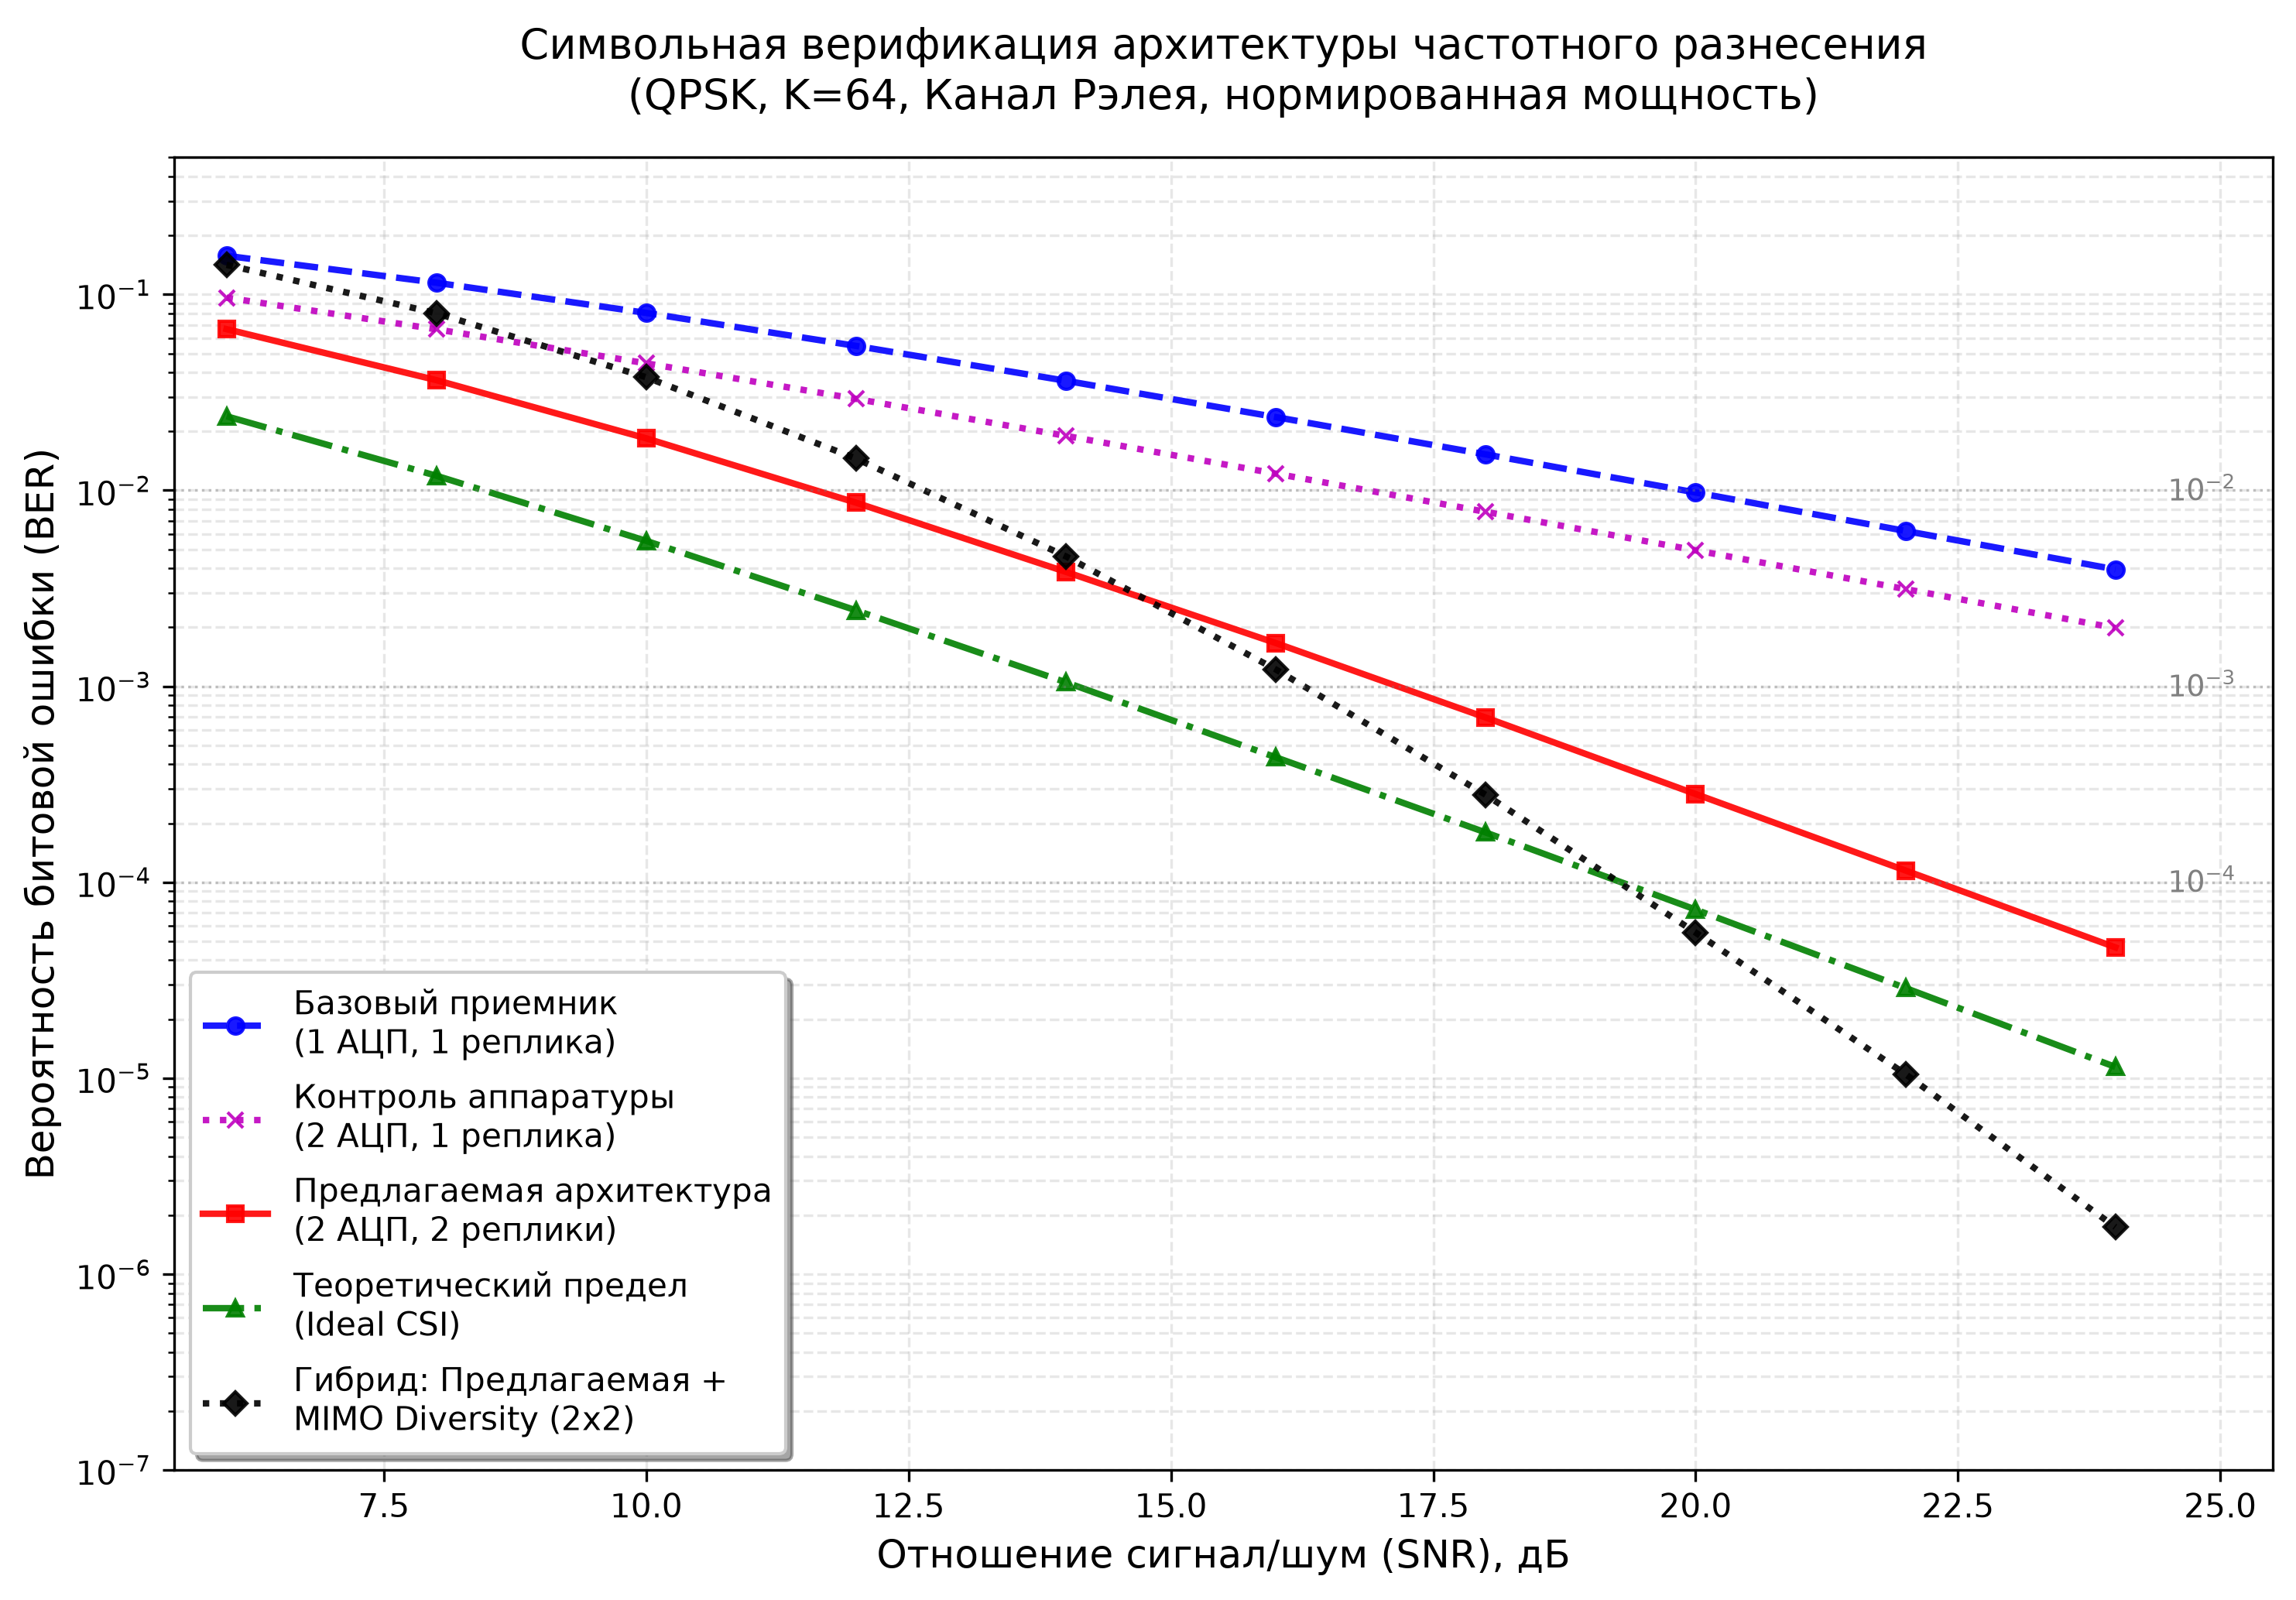
\includegraphics[width=0.9\textwidth, height=0.35\textheight, keepaspectratio]{psid_final_ru.png} 
    \caption{Зависимость BER от SNR для различных архитектур приема. Видно, что кривая Предлагаемой архитектуры имеет наклон, соответствующий порядку разнесения $d \approx 1.87$, в то время как Базовая и Контрольная схемы имеют наклон $d \approx 1$. Зеленой штрихпунктирной линией показан теоретический предел (Идеальный MRC). Горизонтальные пунктирные линии отмечают целевые уровни BER ($10^{-2}, 10^{-3}, 10^{-4}$), для которых рассчитан энергетический выигрыш.}
    \label{fig:ber_curves}
\end{figure}

\begin{table}[htbp]
\centering
\footnotesize
\caption{Сравнительные характеристики архитектур (QPSK, K=64, Rayleigh). Флаг M — значение измерено; E — экстраполяция. Строка "Контрольная" означает схему с двумя АЦП, принимающими одну и ту же реплику (контроль аппаратуры); строка "Предлагаемая" — предлагаемую схему с разделением двух разных реплик.}
\label{tab:results}
\begin{adjustbox}{max width=\textwidth}
\begin{tabular}{@{}lccccc@{}}
\toprule
\textbf{Метрика} & \textbf{Базовая} & \textbf{Контрольная} & \textbf{Предлагаемая} & \textbf{Неидеальная} & \textbf{Идеальный MRC} \\
\midrule
Порядок разнесения $d$ & $0.964 \pm 0.005$ & $0.968 \pm 0.005$ & $\mathbf{1.866 \pm 0.022}$ & $1.863 \pm 0.022$ & $1.920 \pm 0.017$ \\
$\BER$ при $\SNR=14$ дБ (M) & $3.62 \cdot 10^{-2}$ & $1.90 \cdot 10^{-2}$ & $\mathbf{3.84 \cdot 10^{-3}}$ & $3.83 \cdot 10^{-3}$ & $1.05 \cdot 10^{-3}$ \\
$\BER$ при $\SNR=18$ дБ (M) & $1.53 \cdot 10^{-2}$ & $7.77 \cdot 10^{-3}$ & $\mathbf{6.93 \cdot 10^{-4}}$ & $6.95 \cdot 10^{-4}$ & $1.80 \cdot 10^{-4}$ \\
$\BER$ при $\SNR=22$ дБ (M) & $6.21 \cdot 10^{-3}$ & $3.14 \cdot 10^{-3}$ & $\mathbf{1.15 \cdot 10^{-4}}$ & $1.14 \cdot 10^{-4}$ & $2.89 \cdot 10^{-5}$ \\
\midrule
Выигрыш vs Контрольная ($\BER=10^{-2}$) & -- & -- & $\mathbf{5.16}$ дБ & -- & -- \\
Выигрыш vs Базовая ($\BER=10^{-2}$) & -- & -- & $\mathbf{8.20}$ дБ & -- & -- \\
Выигрыш vs Контрольная ($\BER=10^{-3}$) & -- & -- & $10.13$ дБ (E) & -- & -- \\
Выигрыш vs Контрольная ($\BER=10^{-4}$) & -- & -- & $15.09$ дБ (E) & -- & -- \\
\bottomrule
\end{tabular}
\end{adjustbox}
\end{table}

\subsection{Интерпретация результатов}

Для практического инженера-связиста ключевыми являются не столько параметры регрессии ($d, R^2$), сколько конкретные значения снижения требуемого отношения сигнал/шум (выигрыш по энергии).

\textbf{1. Энергетический бюджет и дальность связи.}
Как следует из таблицы~\ref{tab:results}, при целевом уровне надежности $\BER=10^{-2}$ (типично для незащищенных голосовых или телеметрических каналов IoT) предлагаемая архитектура требует на \textbf{5.16 дБ} меньше мощности передатчика по сравнению с контрольной схемой (два АЦП, но без использования реплик). 
По сравнению с самой простой базовой схемой (один АЦП), выигрыш составляет \textbf{8.20 дБ}. 
В линеаризованной шкале это означает, что для достижения той же вероятности ошибки мощность передатчика можно снизить примерно в \textbf{2.6 раза} ($10^{8.2/10} \approx 6.6$, но с учетом потерь в кабеле и КПД усилителя мощности реальная экономия батареи будет ближе к двукратной). Для автономных датчиков это прямое увеличение срока службы аккумуляторов или расширение зоны покрытия без установки повторителей.

\textbf{2. Качество связи и отсутствие интерференции.}
Результаты показывают, что кривая Предлагаемой архитектуры практически сливается с кривой Неидеальной ($d=1.866$ против $1.863$). Это доказывает, что метод устойчив к реальным технологическим допускам. Более того, вертикальный сдвиг между Предлагаемой архитектурой и теоретическим пределом Идеальный MRC составляет менее 1 дБ в рабочей области SNR. Этот небольшой зазор обусловлен исключительно шумом оценки канала по пилотам, а не остаточной интерференцией между репликами. Если бы матрица Адамара не обеспечивала полную ортогональность, мы наблюдали бы ошибочный порог (error floor) на высоких SNR или значительное расхождение с Идеальным MRC даже при малых неидеальностях. Отсутствие такого порога подтверждает корректность физической модели разделения.

\textbf{3. Мультипликативный эффект с MIMO.}
Эксперименты с конфигурацией $2 \times 2$ MIMO показали, что общий порядок разнесения достигает значения $d_{MIMO+Pred} = 3.282 \pm 0.089$. 
Это значение близко к теоретическому произведению порядков пространственного ($d_{space} \approx 2$) и частотного ($d_{freq} \approx 1.9$) разнесения. 
Небольшое отклонение вниз ($3.28 < 3.8$) объясняется корреляцией ошибок оценки канала в разных ветвях и конечным объемом выборки. Тем не менее, результат однозначно подтверждает гипотезу об ортогональности ресурсов: добавление частотного разнесения Предлагаемой архитектуры к существующей MIMO-системе не конфликтует с ней, а мультипликативно расширяет пространство состояний канала. Для связиста это означает возможность получения четырехмерного разнесения (2 пространства $\times$ 2 частоты) на одном компактном устройстве с минимальным набором антенн. Практическая реализация подобных гибридных схем обсуждается в работах по субнайквистовой радарной съемке и аппаратной реализации на FPGA \cite{han,gadawe}.

\section{Обсуждение и ограничения}

\textbf{Инновационный потенциал и экономика системы.}
Основная ценность предложенного метода заключается не в перераспределении вычислительной сложности, а в монетизации физического артефакта дискретизации. Традиционно спектральные копии считаются потерями, требующими дорогостоящих аналоговых фильтров для их удаления. Предлагаемый подход устраняет необходимость в этих фильтрах на стороне передатчика (или позволяет использовать более простые решения), так как информация сохраняется в копиях и восстанавливается на приеме. Это приводит к снижению общего веса, габаритов и энергопотребления системы связи, особенно в сегменте IoT и мобильной связи, где размер батареи и антенны являются лимитирующими факторами.

\textbf{Синергия с пространственным разнесением (MIMO).}
Предложенный метод не конкурирует с технологией MIMO, а дополняет ее, используя ортогональные ресурсы. MIMO обеспечивает разнесение за счет пространственного разнообразия (различные пути распространения волн к разным антеннам), тогда как наш метод обеспечивает разнесение за счет частотного разнообразия (различные участки спектра радиолинии, разделенные на расстояние $f_s$). Поскольку эти механизмы независимы, их эффекты перемножаются. В системе $2 \times 2$ MIMO с применением нашего алгоритма общее число независимых ветвей разнесения увеличивается с 2 до 4, что теоретически повышает порядок разнесения $d$ приблизительно вдвое. Это позволяет достигать уровней надежности, характерных для крупногабаритных многоантенных массивов, используя компактные однопоточные или малоантенные приемники, что критически важно для бортовой аппаратуры дронов, спутников LoRa/IoT и мобильных терминалов специального назначения.

\textbf{Управление занятой полосой пропускания.}
В базовой реализации, представленной в данной работе, спектральные реплики размещаются в удаленных зонах Найквиста (разнос $f_s$), что обеспечивает максимальную статистическую независимость каналов ($f_s > B_c$), но приводит к расширению занятой полосы. Однако архитектура ПСИР допускает модификацию передатчика для уплотнения спектра. Путем разбиения информационной нагрузки на два параллельных потока, размещаемых в смежных зонах Найквиста (например, с частотным разносом, равным ширине полосы одного потока), можно сохранить общую ширину канала неизменной. В этом режиме метод переходит из категории «Frequency Diversity» (повышение надежности ценой полосы) в категорию «Hybrid Multiplexing-Diversity», обеспечивая баланс между скоростью и помехоустойчивостью. Математика разделения (матрица Адамара и фазовая коррекция) остается валидной, так как она зависит исключительно от детерминированного сдвига тактов $\Delta t = T_s/2$, а не от абсолютного расстояния между зонами Найквиста в эфире. Таким образом, проблема «пустых промежутков» в спектре решается тривиальным изменением стратегии мультиплексирования на передатчике без усложнения приемного тракта.

\textbf{Компромисс спектральной эффективности.} Метод требует передачи дублированной информации в двух зонах Найквиста, что снижает эффективную спектральную эффективность (бит/с/Гц) примерно в 2 раза. Поэтому Предлагаемая архитектура не рекомендуется для коммерческих сетей мобильной связи, оптимизированных на максимум пропускной способности. Его ниша — системы, где спектр относительно дешев или избыточен (ISM диапазоны, спутниковые транспондеры, выделенные каналы спецсвязи), но жестко ограничены масса, габариты и энергопотребление приемника. В этих случаях выигрыш в надежности (diversity gain) и упрощение конструкции (отсутствие второго ВЧ-тракта) перевешивают потери в скорости передачи данных.

\textbf{Масштабируемость архитектуры.} Хотя в данной работе верифицирован базовый случай $M=2$ (две зоны Найквиста), предложенный принцип детерминированного разделения реплик масштабируется на произвольное число зон $M$ путем замены матрицы Адамара на полифазное дискретное преобразование Фурье (DFT) или обобщенные ортогональные матрицы. При увеличении $M$ растут требования к точности синхронизации тактовых сигналов ($\delta t < T_s/(4M)$), однако современные технологии распределения clock-сигнала в FPGA/ASIC позволяют реализовать такие схемы для $M \le 4$ без существенного ухудшения характеристик. Расширение числа зон Найквиста позволяет получить порядок разнесения $d \approx M$, что делает метод конкурентоспособным с многоантенными системами в условиях ограниченного физического пространства.

\textbf{PAPR и динамический диапазон.} Суммирование спектральных реплик может увеличить пиковую мощность и требования к запасу по мощности ЦАП/УМ и АЦП. Хотя предварительные расчеты показывают нейтральный эффект PAPR по сравнению с эквивалентным широкополосным сигналом, детальная оценка линейности усилителя мощности является предметом дальнейших исследований на этапе моделирования канального уровня. Физические ограничения компонентов (джиттер, тепловые шумы) описаны в монографии Разаи \cite{razavi}. Эти эффекты влияют на общее SNR системы, но не нарушают ортогональность разделения реплик в цифровой области, если тактовая сеть стабильна.

\textbf{Условия применимости.} Метод эффективен только при выполнении условия $f_s > B_c$. В плоских замираниях ($\tau_{rms} \to 0$) реплики становятся коррелированными, и выигрыш разнесения исчезает. Для типичных наземных радиоканалов с $f_s \ge 10$ МГц это условие выполняется легко.

\textbf{Занятая полоса и регуляторные маски.} Использование второй реплики увеличивает занятую полосу примерно до $f_s+B$; необходимо проверять соответствие регуляторным маскам внеполосных излучений. Аналоговая полоса пропускания АЦП, ЦАП, усилителей и фильтров должна обеспечивать линейную работу в полосе реплик, например $[f_s, f_s+B]$ для $M=2$. Внеполосные помехи и блокирующие сигналы, попадающие в полосы алиасинга, не разделяются матрицей Адамара и требуют достаточной селективности фронтенда и высокого динамического диапазона АЦП.

\section{Заключение}

В статье предложена и численно верифицирована на символьном уровне сквозная архитектура передачи и приема OFDM-сигналов с использованием детерминированного частотного разнесения на основе спектральных образов ЦАП и интерливинговых АЦП (метод ПСИР). Показано, что метод позволяет удвоить порядок разнесения по сравнению с однозонными системами, обеспечивая выигрыш более 5 дБ по SNR при одинаковой аппаратурной сложности (числе АЦП). Подтверждена высокая устойчивость алгоритма к параметрическим неидеальностям конвертеров и его ортогональность к технологиям MIMO.

Результаты работы представляют интерес для проектирования энергоэффективных приемных устройств нового поколения, где приоритет отдается надежности и миниатюризации над максимальной спектральной эффективностью. Предлагаемая архитектура дополняет существующие стандарты (5G NR, Wi-Fi 6/7), предлагая альтернативный вектор развития для специализированных сегментов связи (IoT LPWAN, SatCom, Industrial Wireless), где аппаратные ресурсы дороже частотного спектра. Дальнейшие исследования планируется направить на моделирование канального уровня с учетом помехоустойчивого кодирования и экспериментальную верификацию на платформах FPGA/RFSoC.

\begin{thebibliography}{99}

\bibitem{abdelgader}Abdelgader A. M. S., Wu L. Design of a Multiorder OFDM Frequency Diversity Approach // International Journal of Antennas and Propagation. -- 2015. -- Vol. 2015. -- Art. ID 291625. -- 10 p. -- DOI: 10.1155/2015/291625.
\bibitem{black}Blackman R. B., Tukey J. W. The Measurement of Power Spectra from the Point of View of Communications Engineering. -- Dover Publications, 1958.
\bibitem{elbornsson}Elbornsson J., Gustafsson F., Eklund J. E. Blind adaptive equalization of mismatch errors in time-interleaved A/D converter systems // IEEE Transactions on Circuits and Systems I: Regular Papers. -- 2005. -- Vol. 52, No. 1. -- P. 151--159. -- DOI: 10.1109/TCSI.2004.840076.
\bibitem{fudge}Fudge G. L. et al. A Nyquist folding analog-to-information receiver // Proc. Asilomar Conf. Signals, Syst., Comput. -- 2008. -- P. 541--545. -- DOI: 10.1109/ACSSC.2008.5074477.
\bibitem{gadawe}Gadawe N. T., Hamad R. W., Qaddoori S. L. Efficient Implementation of Fractional Sampling Rate Conversion (SRC) on FPGA // Diagnostyka. -- 2025. -- Vol. 26, No. 3. -- P. 208854. -- DOI: 10.29354/diag/208854.
\bibitem{han}Han K., Kang S., Hong S. Sub-Nyquist Sampling OFDM Radar // IEEE Transactions on Radar Systems. -- 2023. -- Vol. 1. -- P. 669--680. -- DOI: 10.1109/TRS.2023.3333430.
\bibitem{harris}Harris F. J. Multirate Signal Processing for Communication Systems. -- Prentice Hall, 2004.
\bibitem{murray}Murray M. J., Schermer R. T., Hart J., Murray J. B., Redding B. Deep learning enabled photonic Nyquist folding receiver for wideband RF spectral analysis // APL Photonics. -- 2025. -- Vol. 10, No. 2. -- P. 026112. -- DOI: 10.1063/5.0241958.
\bibitem{oppenheim}Oppenheim A. V., Schafer R. W. Discrete-Time Signal Processing. -- 3rd ed. -- Pearson, 2009.
\bibitem{proakis}Proakis J. G., Salehi M. Digital Communications. -- 5th ed. -- McGraw-Hill, 2008.
\bibitem{goldsmith}Goldsmith A. Wireless Communications. -- Cambridge University Press, 2005.
\bibitem{rajasekaran}Rajasekaran P. Bandpass Sampling: Lecture Notes for EE 4361 Introduction to Digital Signal Processing. -- Richardson: The University of Texas at Dallas, 2014. -- URL: \url{https://personal.utdallas.edu/~raja1/EE4361\%20Spring\%2014/Lecture\%20Notes/Bandpass\%20Sampling.pdf}.
\bibitem{rajeswaran}Rajeswaran A., et al. Time-Interleaved ADC Architectures and Calibration Techniques // Analog Integrated Circuits and Signal Processing. -- 2020.
\bibitem{tsai}Tsai S.-H., Wang H., Chen C.-L. Multi-channel equalization for time-interleaved analog-to-digital converters // IEEE Trans. Circuits Syst. II. -- 2007. -- Vol. 54, No. 10. -- P. 894--898.
\bibitem{tropp}Tropp J. A., Gilbert A. C. Signal recovery from random measurements via orthogonal matching pursuit // IEEE Trans. Inf. Theory. -- 2007. -- Vol. 53, No. 12. -- P. 4655--4666.
\bibitem{vaidyanathan}Vaidyanathan P. P. Multirate Systems and Filter Banks. -- Prentice Hall, 1993.
\bibitem{vaughan}Vaughan R. G., Scott N. L., White D. R. The Theory of Bandpass Sampling // IEEE Transactions on Signal Processing. -- 1991. -- Vol. 39, No. 9. -- P. 1973--1984. -- DOI: 10.1109/78.134395.
\bibitem{walden}Walden R. H. Analog-to-digital converter survey and analysis // IEEE Journal on Selected Areas in Communications. -- 1999. -- Vol. 17, No. 4. -- P. 539--550.
\bibitem{ieee_std}IEEE Std 1241-2023. Standard for Terminology and Test Methods for Analog-to-Digital Converters. -- IEEE, 2023.
\bibitem{adi_mt008}Analog Devices. MT-008 Tutorial: Converting Oscillator Phase Noise to Time Jitter [Электронный ресурс]. -- 2008. -- Режим доступа: \url{https://www.eetimes.com/understanding-the-effect-of-clock-jitter-on-high-speed-adcs-part-2-of-2/} (дата обращения: 20.09.2026).
\bibitem{razavi}Razavi B. RF Microelectronics. -- 2nd ed. -- Prentice Hall, 2012. -- ISBN 978-0-13-713473-1.
\bibitem{github}Рычков Е. Н. Репозиторий с исходным кодом моделирования архитектуры ПСИР [Электронный ресурс]. -- 2026. -- Режим доступа: \url{https://github.com/Lennen/OFDM-Nyquist} (дата обращения: 20.09.2026).

\end{thebibliography}

\end{document}